\documentclass{beamer}
 
\usepackage{fontawesome}
\usepackage[utf8]{inputenc}
\usepackage{hyperref} 
\usepackage{tikz}

\usetikzlibrary{calc}


\usetheme{Madrid}
\setbeamertemplate{itemize subitem}[square]

\title{A very informal introduction to Git}
\author{Federico Galatolo}
\date{}
\titlegraphic{\includegraphics[width=.3\textwidth,height=.2\textheight]{imgs/git-logo.eps}}


\begin{document}

\frame{\titlepage}

\begin{frame}
    \frametitle{What is not git?}
    \begin{figure}
        \includegraphics[scale=0.1]{imgs/cloud.png}
    \end{figure}
    \begin{itemize}
        \item Dropbox
        \item Google Drive
        \item iCloud
        \item ...
    \end{itemize}
\end{frame}

\begin{frame}
    \frametitle{What is git?}
    \begin{figure}
        \includegraphics[scale=0.5]{imgs/git-logo.eps}
    \end{figure}
    \hfill \\\hfill \\\hfill \\
	Git is VCS (Version Control System). \\
	\hfill \\
	VCS are about the \textbf{changes} not the \textbf{files}\\
\end{frame}

\begin{frame}
    \frametitle{Git is more than a VCS}
    \begin{figure}
        \includegraphics[scale=0.3]{imgs/git-distributed.png}
    \end{figure}
    \hfill \\\hfill \\
    Git is a \textbf{distributed} VCS.\\
    \hfill \\
    Each participant can have a different view of the state of the project.\\
\end{frame}

\begin{frame}[fragile]
    \begin{figure}
        \includegraphics[scale=0.3]{imgs/repo.png}
    \end{figure}
    \frametitle{Repository}
    A Repository (or ``repo'') is a data structure containing all project's files and history.\\
    \hfill \\
    You can clone a remote repo with the \texttt{clone} command:
    \hfill \\ \hfill \\
    \texttt{git clone <repo url>}
\end{frame}

\begin{frame}
    \frametitle{Special files}
    In a repo you can notice some files starting with \texttt{.git}\\
    \hfill \\
    Those are special files and folders used to store the project history and to instruct git.
    \hfill \\\hfill \\
    \begin{description}
        \item[.git] A folder containing the project history (do not touch!)
        \item[.gitignore] A file containing ignoring rules
        \item[.gitmodules] A file containing submodules information  
    \end{description} 
\end{frame}

\begin{frame}
    \frametitle{Commit}
    \begin{center}
    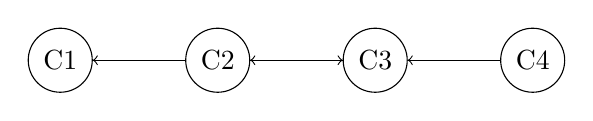
\begin{tikzpicture}[
        node/.style={
            circle, 
            draw,
            radius=1cm,
        }
    ]

    \node (C1) at (0,0) [node] {C1};
    \node (C2) at (2,0) [node] {C2};
    \node (C3) at (4,0) [node] {C3};
    \node (C4) at (6,0) [node] {C4};

    \draw [->] (C2) -- (C1);
    \draw [->] (C3) -- (C2);
    \draw [->] (C2) -- (C3);
    \draw [->] (C4) -- (C3);
    
    

    \end{tikzpicture}
\end{center}
    \hfill \\
    A \textbf{commit} is a \textbf{snapshot} of the project in a given time.\\
    \hfill \\
    Commits are \textbf{immutable} and represent a transition from a state to another.\\
    \hfill \\
    The commits are atomic units of modification within a project.\\
    \hfill \\
    A commit is uniquely identified by its \textbf{hash} 
\end{frame}


\begin{frame}
    \frametitle{How to commit}
    A git commit is a two-stages process.\\
    \begin{itemize}
        \item Add files to the staging environment
        \item Commit the changes
    \end{itemize}
    \begin{center}
    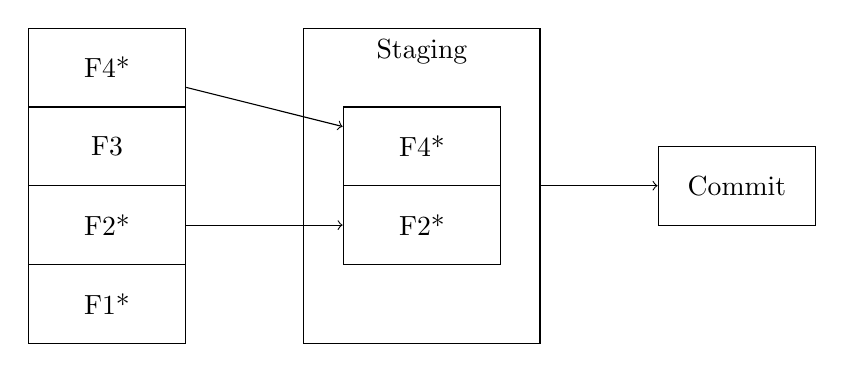
\begin{tikzpicture}[
        node/.style={
            circle, 
            draw,
            radius=1cm,
        },
        file/.style={
            rectangle, 
            draw,
            minimum width=2cm,
            minimum height=1cm,
        },
        staging/.style={
            rectangle, 
            draw,
            minimum width=3cm,
            minimum height=4cm,
        },
    ]

    \foreach \x in {1,2,4}{
        \node (f\x) at (0,\x) [file] {F\x*};
    }
    \node (f3) at (0,3) [file] {F3};

    \pause

    \node (s) at (4, 2.5) [staging] {};
    \node [] at  ($(s.north) + (0,-0.3)$)  {Staging};

    \pause

    \node (s4) at (4,3) [file] {F4*};
    \node (s2) at (4,2) [file] {F2*};
    
    \draw [->] (f4) -- (s4);
    \draw [->] (f2) -- (s2);
    
    \pause

    \node (c) at (8, 2.5) [file] {Commit};
    \draw [->] (s) -- (c);
    
    \onslide<1->
    \end{tikzpicture}
\end{center}
\end{frame}


\begin{frame}
    \frametitle{How to commit(2)}
    \begin{itemize}
        \item Check modified files 
        \begin{itemize}
            \item \texttt{git status}
        \end{itemize}
        \item Check commits history
        \begin{itemize}
            \item \texttt{git log}
        \end{itemize}
        \item Add files to the staging environment
        \begin{itemize}
            \item \texttt{git add file/folder}
        \end{itemize}
        \item Commit the changes
        \begin{itemize}
            \item \texttt{git commit -m "commit message"}
        \end{itemize}
    \end{itemize}
    \hfill \\
    \begin{center}
    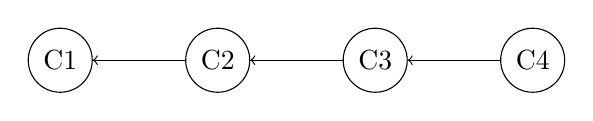
\begin{tikzpicture}[
        node/.style={
            circle, 
            draw,
            radius=1cm,
        }
    ]

    \node (C1) at (0,0) [node] {C1};
    \node (C2) at (2,0) [node] {C2};    

    \draw [->] (C2) -- (C1);
    
    \pause
    \node (C3) at (4,0) [node] {C3};
    \draw [->] (C3) -- (C2);

    \pause

    \node (C4) at (6,0) [node] {C4};
    \draw [->] (C4) -- (C3);
    
    \onslide<1->
    \end{tikzpicture}
\end{center}
\end{frame}


\begin{frame}
    \frametitle{HEAD}
    \begin{center}
    \begin{tikzpicture}[
        node/.style={
            circle, 
            draw,
            radius=1cm,
        },
        head/.style={
            rectangle, 
            draw,
            minimum width=2cm,
            minimum height=1cm,
        },
    ]

    \node (C1) at (0,0) [node] {C1};
    \node (C2) at (2,0) [node] {C2};    

    \draw [->] (C2) -- (C1);
    
    \only<1>{
        \node (h1) at (2, -2) [head] {HEAD};
        \draw [->] (h1) -- (C2);
    }

    \pause
    \node (C3) at (4,0) [node] {C3};
    \draw [->] (C3) -- (C2);
    
    \only<2>{
        \node (h2) at (4, -2) [head] {HEAD};
        \draw [->] (h2) -- (C3);
    }
    \pause

    \node (C4) at (6,0) [node] {C4};
    \draw [->] (C4) -- (C3);

    \only<3>{
        \node (h3) at (6, -2) [head] {HEAD};
        \draw [->] (h3) -- (C4);
    }
    
    \onslide<1->
    \end{tikzpicture}
\end{center}
    \hfill \\
    \texttt{HEAD} is a git variable that points to the most recent commit.
\end{frame}

\begin{frame}
    \frametitle{Git superpowers}
    Your main git superpower is:
    \begin{itemize}
        \item \texttt{git reset <NEW\_HEAD>}
    \end{itemize}
    \hfill \\
    With this command you can change \texttt{HEAD} and make it point to a different commit.
    \begin{itemize}
        \item Change HEAD \textbf{without} changing the files
        \begin{itemize}
            \item \texttt{git reset <NEW\_HEAD>}
        \end{itemize}
        \item Change HEAD \textbf{changing} the files
        \begin{itemize}
            \item \texttt{git reset --hard <NEW\_HEAD>}
        \end{itemize}
    \end{itemize}
\end{frame}


\begin{frame}
    \frametitle{Git superpowers(2)}
    For example with:
    \begin{itemize}
        \item \texttt{git reset --hard C2}
    \end{itemize}
    \begin{center}
    \begin{tikzpicture}[
        node/.style={
            circle, 
            draw,
            radius=1cm,
        },
        head/.style={
            rectangle, 
            draw,
            minimum width=2cm,
            minimum height=1cm,
        },
    ]

    \node (C1) at (0,0) [node] {C1};
    \node (C2) at (2,0) [node] {C2};
    \node (C3) at (4,0) [node] {C3};
    \node (C4) at (6,0) [node] {C4};

    \draw [->] (C3) -- (C2);
    \draw [->] (C4) -- (C3);
    \draw [->] (C2) -- (C1);
    \only<1>{        
        \node (h1) at (6, -2) [head] {HEAD};
        \draw [->] (h1) -- (C4);
    }

    \only<2>{
        \node (h2) at (2, -2) [head] {HEAD};
        \draw [->] (h2) -- (C2);
    }
    
    \pause
    \onslide<1->

    \end{tikzpicture}
\end{center}
\end{frame}

\begin{frame}
    \frametitle{Git superpowers(3)}
    Don't worry, you are not going to mess it up. \\
    \hfill \\
    If you \texttt{git reset} you will lose in \texttt{git log} all the subsequent commit references. \\
    \hfill \\
    You can retrieve \textbf{all HEAD history} with   
    \begin{itemize}
        \item \texttt{git reflog}
    \end{itemize}
\end{frame}

\begin{frame}
    \frametitle{Learn Git Branching}
    We are going to use a tool called \textit{Learn Git Branching} for the next slides.\\
    This tool allow you to visualize git commands in a graph.\\
    It uses a very simplified subset of git commands:
    \begin{itemize}
        \item \texttt{git commit}
        \begin{itemize}
            \item There is no concept of staging environment nor of files
            \item You can make a commit without message
        \end{itemize}
        \item \texttt{git reset <hash>}
        \begin{itemize}
            \item It uses C1, C2, ... CN as hashes
            \item It always implies the \texttt{--hard} behavior 
        \end{itemize}
        \item \texttt{git clone}
        \begin{itemize}
            \item Treats the repo as it has just been cloned from an identical origin
        \end{itemize}
        \item \texttt{git fakeTeamwork}
        \begin{itemize}
            \item Creates a new commit in remote origin
        \end{itemize}
    \end{itemize}
\end{frame}

\begin{frame}
    \frametitle{Try it yourself!(1)}
    \begin{center}
        \href{https://learngitbranching.js.org/?NODEMO\&command=git\%20commit;git\%20commit}{Exercise 1}
    \end{center}
    \begin{figure}
        \includegraphics[scale=0.4]{imgs/ex1.png}
    \end{figure}
\end{frame}


\begin{frame}
    \frametitle{Branches}
    \begin{center}
    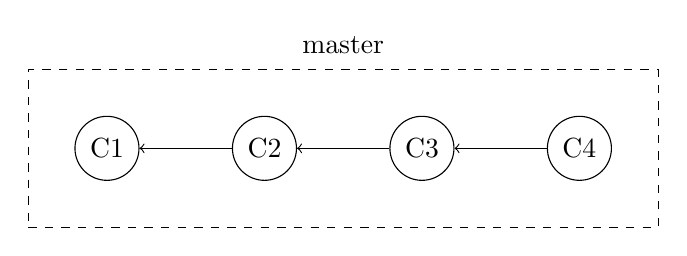
\begin{tikzpicture}[
        node/.style={
            circle, 
            draw,
            radius=1cm,
        },
        branch/.style={
            rectangle, 
            draw,
            minimum width=8cm,
            minimum height=2cm,
            dashed
        },
    ]

    \node (C1) at (0,0) [node] {C1};
    \node (C2) at (2,0) [node] {C2};
    \node (C3) at (4,0) [node] {C3};
    \node (C4) at (6,0) [node] {C4};

    \draw [->] (C2) -- (C1);
    \draw [->] (C3) -- (C2);
    \draw [->] (C4) -- (C3);

    \node (b) at (3, 0) [branch] {};
    \node [] at  ($(b.north) + (0,0.3)$)  {master};

    

    \end{tikzpicture}
\end{center}
    \hfill \\
    A branch is a (semantically significant) collection of commits.\\
    \hfill \\
    As a commit represent an atomic unit of modification, \\
    a branch represent a continuous flow of modifications. \\
    \hfill \\
    A commit is \textbf{always} in a branch. 
\end{frame}

\begin{frame}
    \frametitle{Branches(2)}
    \begin{itemize}
        \item \texttt{git branch}
        \begin{itemize}
            \item Show all the existing branches and the active one (denoted with an asterisk)
        \end{itemize}
        \item \texttt{git branch <branch>}
        \begin{itemize}
            \item Create a new branch called \texttt{<branch>} 
        \end{itemize}
        \item \texttt{git checkout <branch>}
        \begin{itemize}
            \item Switch working on the branch \texttt{<branch>}
        \end{itemize}
        \item \texttt{git checkout -b <branch>}
        \begin{itemize}
            \item Create \texttt{<branch>} and switch working on it 
        \end{itemize}
    \end{itemize}
\end{frame}


\begin{frame}
    \frametitle{Try it yourself!(2)}
    \begin{center}
        \href{https://learngitbranching.js.org/?NODEMO}{Exercise 2}
    \end{center}
    \begin{figure}
        \includegraphics[scale=0.4]{imgs/ex2.png}
    \end{figure}
\end{frame}


\begin{frame}
    \frametitle{Merge(1)}
    You can merge different branches (or even single commits).\\
    Most of the times commits has been pushed in both branches. \\
    \textbf{Don't panic!}
    \begin{center}
    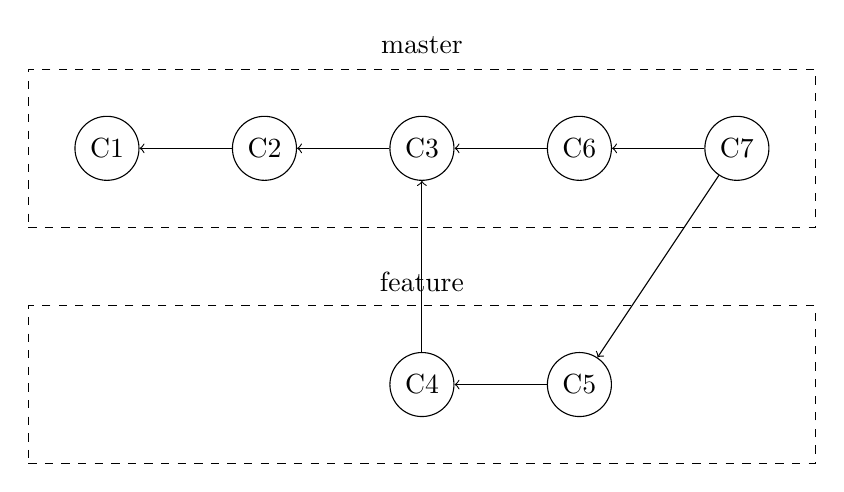
\begin{tikzpicture}[
        node/.style={
            circle, 
            draw,
            radius=1cm,
        },
        branch/.style={
            rectangle, 
            draw,
            minimum width=10cm,
            minimum height=2cm,
            dashed
        },
    ]

    \node (C1) at (0,0) [node] {C1};
    \node (C2) at (2,0) [node] {C2};
    \node (C3) at (4,0) [node] {C3};
    
    \draw [->] (C2) -- (C1);
    \draw [->] (C3) -- (C2);


    \node (b1) at (4, 0) [branch] {};
    \node [] at  ($(b1.north) + (0,0.3)$)  {master};
    
    \pause 

    \node (b2) at (4, -3) [branch] {};
    \node [] at  ($(b2.north) + (0,0.3)$)  {feature};


    \node (C4) at (4,-3) [node] {C4};
    \draw [->] (C4) -- (C3);
    
    \pause 
    \node (C5) at (6,-3) [node] {C5};
    \draw [->] (C5) -- (C4);


    \pause

    \node (C6) at (6,0) [node] {C6};
    \draw [->] (C6) -- (C3);

    \pause

    \node (C7) at (8, 0) [node] {C7};
    \draw [->] (C7) -- (C6);
    \draw [->] (C7) -- (C5);
    

    \onslide<1->
    \end{tikzpicture}
\end{center}
\end{frame}

\begin{frame}
    \frametitle{Merge(2)}
    Don't worry, git auto-merge is smart.\\
    \hfill \\
    If the commits changed \textbf{different files} the merge is \textbf{without conflicts}.\\
    \hfill \\
    If the commits changed \textbf{different sections of the same files} the merge is \textbf{without conflicts}.\\
    \hfill \\
    If the commits changed the \textbf{same sections} of the \textbf{same files} (at least once) the commit is \textbf{with conflict} \hfill \\
    \begin{itemize}
        \item \texttt{git merge <branch>}
        \begin{itemize}
            \item Merges \texttt{<branch>} in the active branch
        \end{itemize}
        \item \texttt{git merge --abort}
        \begin{itemize}
            \item Abort the merge and restore everything as it was before \texttt{git merge}
        \end{itemize}
    \end{itemize}
\end{frame}


\begin{frame}
    \frametitle{Try it yourself!(3)}
    \begin{center}
        \href{https://learngitbranching.js.org/?NODEMO\&command=git\%20commit;git\%20checkout\%20-b\%20feature;git\%20commit;git\%20commit;git\%20checkout\%20master;git\%20commit;git\%20checkout\%20feature}{Exercise 3}
    \end{center}
    \begin{figure}
        \includegraphics[scale=0.3]{imgs/ex3.png}
    \end{figure}
\end{frame}


\begin{frame}
    \frametitle{Merge(3)}
    Handling conflicts is pretty easy.\\
    When a conflict is detected git puts in the place of the conflict:
    \hfill \\
    \texttt{\\
    Some non-conflicting text \\
    <<<<<<< HEAD \\
    CONFLICTING PORTION COMING FROM HEAD \\
    ======= \\
    CONFLICTING PORTION COMING FROM bugfix \\
    >>>>>>> bugfix \\
    Some other non-conflicting text \\
    }
    \hfill \\
    Is then up to you keep the portions that you want and then \texttt{git add} and \texttt{git commit} the changes
\end{frame}


\begin{frame}
    \frametitle{Remotes}
    Git is distributed. \\
    \hfill \\
    A \texttt{remote} is a reference to a remote instance of the repository.\\
    The default \texttt{remote} is called \texttt{origin}.\\
    If you \texttt{clone} a repository then \texttt{origin} points to the cloned repo.\\
    \hfill \\
    \begin{itemize}
        \item \texttt{git fetch <remote> <branch>}
        \begin{itemize}
            \item Fetch the commits from branch \texttt{<branch>} of \texttt{<remote>} in the local branch \texttt{<remote>}/\texttt{<branch>}
        \end{itemize}
        \item \texttt{git pull <remote> <branch>}
        \begin{itemize}
            \item Fetch the commits from branch \texttt{<branch>} of \texttt{<remote>} and \textbf{merge} them in the local \texttt{<branch>}
        \end{itemize}
        \item \texttt{git push <remote> <branch>}
        \begin{itemize}
            \item Push the state of the local \texttt{branch} to the \texttt{origin} branch \texttt{branch} 
        \end{itemize}
    \end{itemize}
\end{frame}


\begin{frame}
    \frametitle{Try it yourself!(4)}
    \begin{center}
        \href{https://learngitbranching.js.org/?NODEMO\&command=git\%20commit;git\%20checkout\%20-b\%20feature;git\%20clone;git\%20fakeTeamwork\%20feature;git\%20fakeTeamwork\%20feature;git\%20checkout\%20master;git\%20commit}{Exercise 4}
    \end{center}
    \begin{figure}
        \includegraphics[scale=0.3]{imgs/ex4.png}
    \end{figure}
    \begin{center}
        you can not use \texttt{git pull}
    \end{center}
\end{frame}



\begin{frame}
    \frametitle{Git tags}
    Tags are a way to point specific points in time (commits) that represent milestones.\\
    \hfill \\
    \begin{itemize}
        \item \texttt{git tag <tag> <commit>}
        \begin{itemize}
            \item Tags \texttt{<commit>} with the tag \texttt{<tag>}
            \item The default commit is HEAD
        \end{itemize}
        \item \texttt{git checkout <tag>}
        \begin{itemize}
            \item Check out the tag \texttt{<tag>}
        \end{itemize}
        \item \texttt{git push <remote> <tag>}
        \begin{itemize}
            \item Push the (newly created) tag \texttt{<tag>} to the remote \texttt{<remote>}
        \end{itemize}
        \item \texttt{git push <remote> --tags}
        \begin{itemize}
            \item Push all the (newly created) tags to the remote \texttt{<remote>}
        \end{itemize}
    \end{itemize}
\end{frame}

\begin{frame}
    \frametitle{Cherry picking}
    \begin{figure}
        \includegraphics[scale=0.25]{imgs/pick.jpg}
    \end{figure}
    \hfill \\
    Cherry picking is the action of merging into \texttt{HEAD} some cherry-picked commits.
    \hfill \\
    \begin{itemize}
        \item \texttt{git cherry-pick <commit>}
        \begin{itemize}
            \item Applies the changes from commit \texttt{<commit>} to \texttt{HEAD}
        \end{itemize}
    \end{itemize}
\end{frame}


\begin{frame}
    \frametitle{A successful Git branching model}
    \begin{figure}
        \includegraphics[scale=0.15]{imgs/git-model.png}
    \end{figure}
\end{frame}


\begin{frame}
    \frametitle{GitHub}
    \begin{figure}
        \includegraphics[scale=0.075]{imgs/github-logo.png}
    \end{figure}
    GitHub is git server.\\
    \hfill \\
    \begin{itemize}
        \item over 37 Million Users
        \item over 100 Million Repositories 
        \item Largest source code host in the world
        \item Home of millions of free and open source projects 
    \end{itemize}
\end{frame}

\begin{frame}
    \frametitle{GitHub forks}
    In GitHub there is the concept of \textit{fork}.\\
    A fork is a clone of someone else's repository into yours repositories.\\
    \hfill \\
    \textbf{A fork is not a git clone}\\
    \hfill \\
    After a fork you \textbf{own} an exact copy of a repository.\\
    Copy of which you and only you are the administrator.\\  
\end{frame}

\begin{frame}
    \frametitle{GitHub Pull Requests}
    If you want to ask for the integration of your changes in the forked repository you have to open a \textbf{Pull Request}.\\
    \hfill \\
    In the pull request you have to specify the destination branch (original repository) and the source branch (your repository)  
\end{frame}


\begin{frame}
    \frametitle{That's all folks!}
    \begin{center}
        You can find the slides PDF as well as their \LaTeX \;source code on GitHub. \\
        \hfill \\
        https://github.com/galatolofederico/git-very-informal-introduction
    \end{center}
    \hfill \\
    \hfill \\
    \begin{columns}
        \begin{column}{.5\textwidth}
            \begin{itemize}
                \item [\faEnvelope] federico.galatolo@ing.unipi.it
                \item [\faPaperPlane] @galatolo
            \end{itemize}
        \end{column}
        \begin{column}{.5\textwidth}
            \begin{itemize}
				\item [\faGlobe] \href{https://galatolo.me}{galatolo.me}
                \item [\faGithub] @galatolofederico
            \end{itemize}
        \end{column}
    \end{columns}
\end{frame}


\end{document}
